\chapter{Grundlagen}\label{ch:grundlagen}
Um den Unterschied zwischen modernen cloud native Entwicklungsprozessen und dem Mainframe Entwicklungsprozess darstellen zu können, werden zunächst Begriffe aus dem cloud-native-Umfeld erläutert.
Dabei wird auch auf die Vorteile und Begrifflichkeiten des damit ermöglichten Entwicklungsprozesses eingegangen.
Anschließend werden für die Beantwortung der Forschungsfragen relevante Begriffe des Mainframe-Umfelds beleuchtet.

\section{cloud-native bei DATEV e.G.}\label{sec:cloudnative}
Eine cloud-native Anwendung ist eine speziell für das Cloud-Computing\footnote{Glossar \ref{Glossar}} konzipierte und entwickelte Anwendung.
Oft werden damit Online-Anwendungen und mobile \glqq Apps\grqq entwickelt, für die häufig und hoch frequent neue Features bereitgestellt werden sollen. 
Für solche Anwendungen ist das Architekturpattern der sogenannten \glqq Microservices\grqq, weit verbreitet.
Diese einzelnen, entkoppelten Services sind beispielsweise in Containern paketiert. 
Bekannt geworden ist hier der Ansatz von Docker\footnote{Glossar \ref{Docker Glossar link}}.
DIe Docker Container wird über ein Image beschrieben und beinhalte neben der Anwendung alles das, was die Anwendung an Komponenten zur Laufzeit benötigt, Bibliotheken, Dateien (Kommentar: Quelle https://www.dev-insider.de/was-sind-docker-container-a-597762/ 
Somit kann die Anwend können auf verschiedenen "privat" und "public" Cloud-Umgebungen, auch von unterschiedlichen Anbietern, ausgeführt werden.
Große Anbieter sind hier beispielsweise AWS (Amazon), Google, Microsoft Azure. (Kommentar: Quelle z.B: https://neuhandeln.de/im-ueberblick-die-groessten-anbieter-fuer-cloud-computing/) 
Dort können bereitstehende Services für Datenhaltung, Security, Messaging usw. genutzt werden. 
\cite{.23.2.2020d}\\
Eine moderne cloud-native Anwendung innerhalb der DATEV e.G. machen folgende Dinge aus:
\begin{itemize}
\item \glqq Cloud Foundry\grqq
\item CI/CD-Pipeline
\end{itemize}

\subsection{\glqq Cloud Foundry\grqq}
Bei Cloud Foundry handelt es sich um eine quelloffene Platform-as-a-Service, kurz PaaS.
Platform-as-a-Service, beschreibt neben Insfrastructure-as-a-Service, kurz IaaS und Software-as-a-Service, kurz SaaS, einen Grad an Auslagerung von IT-Systemen in die Cloud.
Im Vergleich zu SaaS, bei der ganze Anwendungen in einer Cloud zur Verfügung stehen, und IaaS, bei der die automatisierte Bereitstellung von Infrastrukturkomponenten wie Netzwerk, Speicher usw. im Fokus steht, stellt eine PaaS-Lösung eine Plattform, die sich neben der Infrastruktur auch um das Betriebssystem, die Middleware und die Laufzeitumgebung kümmert, bereit.\footnote{\cite{ipsaas.25.2.2020}}
Für die Verwaltung von Ressourcen bietet Cloud Foundry eine Weboberfläche, den sogenannten \glqq Marketplace\grqq, an.
In diesem können mit wenigen Mausklicks Schnittstellen zu Services wie Datenbankmanagementsysteme, Messaging- oder Monitorlösungen zur Anwendung hinzugefügt werden.
Diese Schnittstellen, auch \glqq Self-Service\grqq{} oder \glqq Service-Broker\grqq{} genannt, können mittels einer von Cloud Foundry zur Verfügung gestellten API selbst entwickelt werden.
Daneben kümmert sich Cloud Foundry um das Staging der Anwendungen.
D.h. eine Anwendung kann mit den benötigten Komponenten sicher von einer Entwicklungs- in eine QS- bzw. Produktiv-Stage verschoben werden. 
Die notwendigen stagespezifischen Anpassungen werden konfigurativ beigesteuert.
Um eine Anwendung in einer bestimmten Stage bereitzustellen, bietet Cloud Foundry ein Kommandozeileninterface an.
Neben der Bereitstellung können mit diesem Interface beispielsweise Anwendungen auch horizontal skaliert werden.
Um die Breitstellung über mehrere Stages hinweg zu automatisieren kommt bei der DATEV e.G. eine auf Jenkins basierende CI/CD-Pipeline zum Einsatz.
\cite{.23.2.2020c}

\subsection{\glqq CI/CD-Pipeline\grqq}\label{sec:cicd}
\begin{figure}[h]
	\centering
	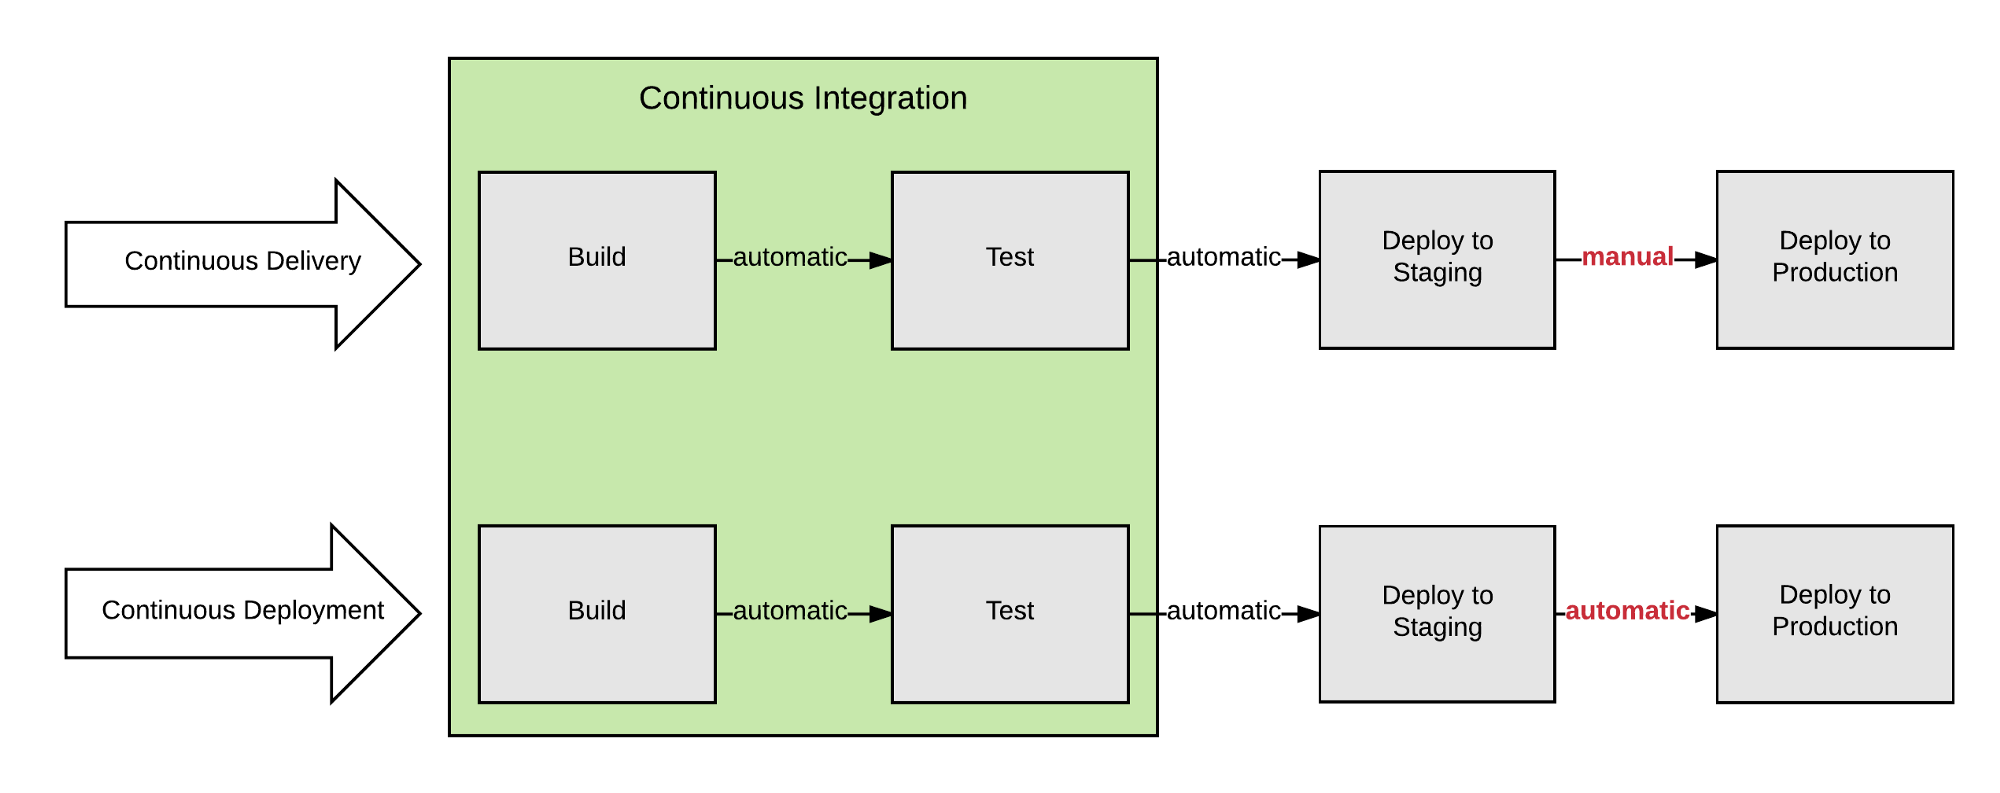
\includegraphics[width=\textwidth]{figures/ci-cd-flow-desktop_1.png}
	\caption{Abgrenzung von Continuous Integration, Continuous Delivery und Continuous Deployment  (Quelle: \cite{.25.2.2020d})}
	\label{fig:cicd}
\end{figure}

CI/CD steht für \glqq Continuous Integration und Continuous Delivery\grqq{} in manchen Fällen auch für \glqq Continuous Integration, Continuous Delivery und Continuous Deployment\grqq{}.
Die einzelnen Begriffe werden im Folgenden erläutert, als Überblick dient Abbildung \ref{fig:cicd}
\paragraph{\glqq Continuous Integration\grqq}~\\
Continous Integration beschreibt einen Prozess, bei dem Änderungen von Entwicklern regelmäßig in eine gemeinsame Codebasis integriert und getestet werden.
In Abbildung \ref{fig:ci} ist der Prozess dargestellt.
\begin{figure}[h]
	\centering
	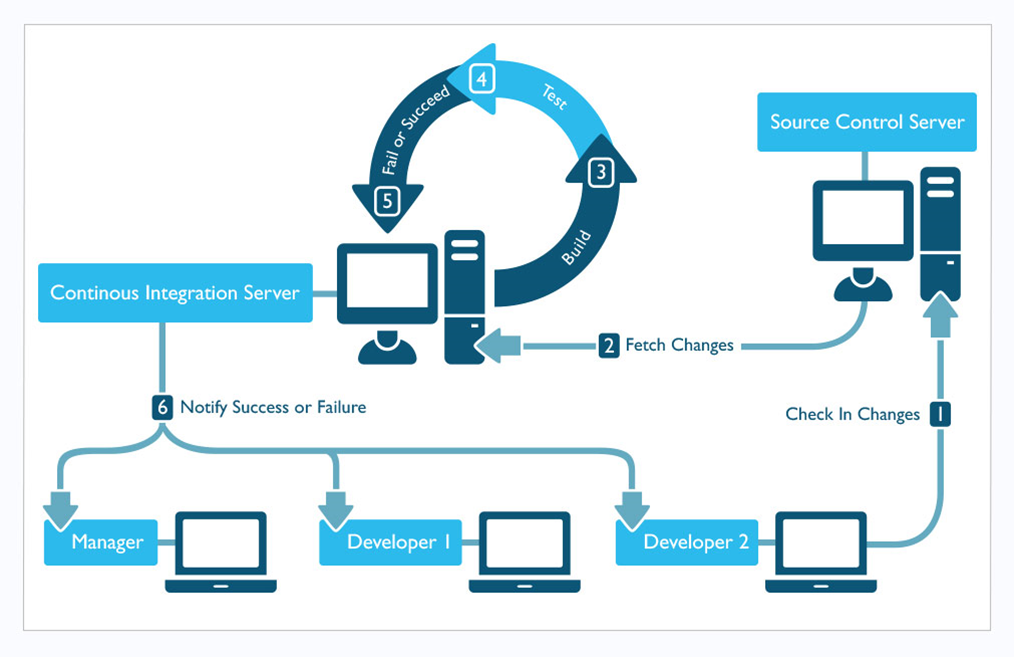
\includegraphics[width=\textwidth]{figures/CI.png}
	\caption{Continuous Integration Prozessaufbau (Quelle: \cite{.25.2.2020e})}
	\label{fig:ci}
\end{figure}
Eine Voraussetzung für den Einsatz von CI ist eine zentrale Sourceverwaltung.
Bei der DATEV e.G. handelt es sich dabei um GIT. (Kommentar: Git-Schreibweise ist noch uneinheitlich)
Nachdem ein Entwickler Änderungen am Code vorgenommen hat, lädt er diese in die Sourceverwaltung hoch.
Dabei kann eine erste Überprüfung des Codes mittels statischer Codeanalyse durchgeführt werden.
Dazu zählt unter anderem die Prüfung vorher definierter Coderichtlinien.
Sind diese erfolgreich, wird ein isolierter CI-Server benachrichtigt.
Dieser Server holt sich den neusten Stand des Quellcodes und baut diesen, um anschließend automatisierte Tests durchzuführen.
Hier liegt der zentrale Vorteil der Automatisierung. 
Bei jedem Bauen wird automatisch überprüft, ob das Ergebnis das erwartete ist.
Voraussetzung dafür ist die oben beschriebene Paketierung der Anwendung mit der Laufzeitumgebung und den benötigten Komponenten. 


Bei den Tests während der Continuous Integration handelt es sich um sogenannte \glqq Unittests\grqq.
Dabei wird anhand vordefinierter Eingangsdaten die Ausgabe bestimmter Funktionen geprüft (Soll-Ist-Vergleich).
Dazu gehört auch die Überprüfung, ob mit Fehlerbedingungen korrekt umgegangen wird.
Dabei werden Abhängigkeiten zu externen Ressourcen, wie beispielsweise einer Datenbank, außen vor gelassen.
Wenn solche Ressourcen dennoch benötigt werden, müssen diese mit Hilfe eines sogenannten \glqq Mocking-Framework\grqq{} simuliert werden.
Schließlich stellt der CI-Server die Ergebnisse dieser Tests (z.B. in einem Jenkins-Dashboard) zur Verfügung. 
\cite{Laster.2017}

\paragraph{\glqq Continuous Delivery\grqq}~\\
Bei Continuous Delivery werden die Änderungen, die vorher auf dem isolierten CI-Server getestet und integriert wurden, in eine Stage, z. B. in die Entwiclungsstage, automatisch übertragen.
Hier werden weitere Tests, wie Integrationstests und Akzeptanztests, durchgeführt.
Am Ende einer Continuous Delivery Pipeline steht ein theoretisch auslieferbarer Stand der Anwendung.
Die Übergabe dieses Standes in die Produktion ist bei Continuous Delivery noch manuell umzusetzen.
\cite{Laster.2017}

\paragraph{\glqq Continuous Deployment\grqq}~\\
Continuous Deployment beschreibt den nächsten Schritt nach Continuous Delivery.
Dabei handelt es sich um die automatisierte Bereitstellung in eine Produktions-Stage.
\cite{Laster.2017}

\section{Mainframe / Großrechner}\label{sec:mainframe}
Im modernen Sprachgebrauch kann ein Großrechner oder auch Mainframe als größte zur Verfügung stehende Serverart betrachtet werden.
Er wird von Unternehmen verwendet, um  kommerzielle Datenbanken, Transaktionsserver und Anwendungen, die einen hohen Grad an Sicherheit und Verfügbarkeit benötigen, zu hosten.
Im Gegensatz zu verteilten Serversystemen, bei denen die Funktionalitäten auf einzelne Server, wie zum Beispiel einen E-Mail-Server, einen Datenbank-Server, einen Web-Server usw. aufgeteilt sind, handelt es sich bei einem Mainframe um ein zentralisiertes System.
Die einzelnen Funktionalitäten werden von sogenannte \glqq Subsysteme\grqq, auch \glqq Middleware\grqq{} genannt, zur Verfügung gestellt. 
Darunter zählen unter anderem Datenbanksysteme und Anwendungsserver.
\cite{Ebbers.2011}

\section{Mainframe Anwendungen bei DATEV e.G.}\label{sec:zosanw}
Das Betriebssystem des IBM Mainframes ist z/OS. (Kommentar: z/OS steht für zero downtime... Quelle -https://www.redbooks.ibm.com/redbooks/pdfs/sg246366.pdf)
Darauf aufbauend benötigen klassische z/OS Anwendungen bestimmte Middleware.
Bei der DATEV e.G. handelt es sich unter anderem um folgende Middlewarekomponenten:

\begin{itemize}
\item Laufzeitumgebung: CICS oder Batch
\item Datenhaltung: VSAM oder Db2
\item Message Queuing: IBM MQ
\end{itemize}

Diese Subsysteme stehen in jeder Stage zur Verfügung.
Eine Stage beschreibt eine isolierte Systemumgebung mit eigenen Subsystemen und Ressourcenverwaltung.
Die DATEV e.G. unterscheidet am Mainframe vier Stages:
\begin{samepage}
\begin{itemize}
\item Testplex:\\
Labor für Änderungen am System, beispielsweise einer neuen Betriebssystemsversion
\item Entwicklung:\\
Implementierung neuer Features und Durchführung kleiner Tests
\item Qualitätssicherung:\\
Durchführung von Integrationstests
\item Produktion:\\
Software, die für den Kunden bereitsteht
\end{itemize}
\end{samepage}

\section{Subsysteme / Middleware}
Für die Beantwortung der Forschungsfragen liegt der Fokus auf dem Erstellen (\glqq Provisionieren \grqq) einer anwendungsspezifischen Laufzeitumgebung mit einer Datenhaltung und Message Queuing auf der Entwicklungs-Stage. (Komemntar Das mit dem Testplex würde ich erst in der Realsierung erwähnen. Es ist aber nicht der Fokus hier)
Als Laufzeitumgebung wird \glqq CICS\grqq, als Datenhaltung \glqq Db2\grqq{} und für das Message Queuing \glqq IBM MQ\grqq{} verwendet.
Wie in Abbildung \ref{fig:archüber} dargestellt ist, sind mehrere Instanzen pro Subsystem möglich.
Bei der DATEV e.G. existiert jedoch nur eine geringe Anzahl an Instanzen pro Subsystem. (Kommentar: hier wäre der Grund interessant, dh. wir könnten Jürgen Miehling oder Maderer mal fragen, warum das so ist. Wenn das so ist, weil der Aufwand, mehrere hinzustellen und zu administrieren, hoch wäre, dann wäre das wieder ein Argument für unsere automatisierte Provisionierung)
Daraus folgt, dass sich, wie in der Problemstellung, Absatz \ref{sec:probstell}, bereits erwähnt, viele Anwendungen die gleichen Entwicklungs-CICS/Db2/MQ Ressourcen teilen. (Kommentar: für CICS und DB2 stimmt das, aber für MQ?) 
Diese Instanzen sind langlebig, und müssen dahingehend gepflegt und gewartet werden, dass sie die Anforderungen für alle Anwendungen, die sich die Ressourcen teilen, abdecken. 

Diese einzelnen Subsysteme werden im Folgenden erläutert, hierzu dient Abbildung \ref{fig:archüber} als Überblick.

\begin{figure}[h!]
\centering
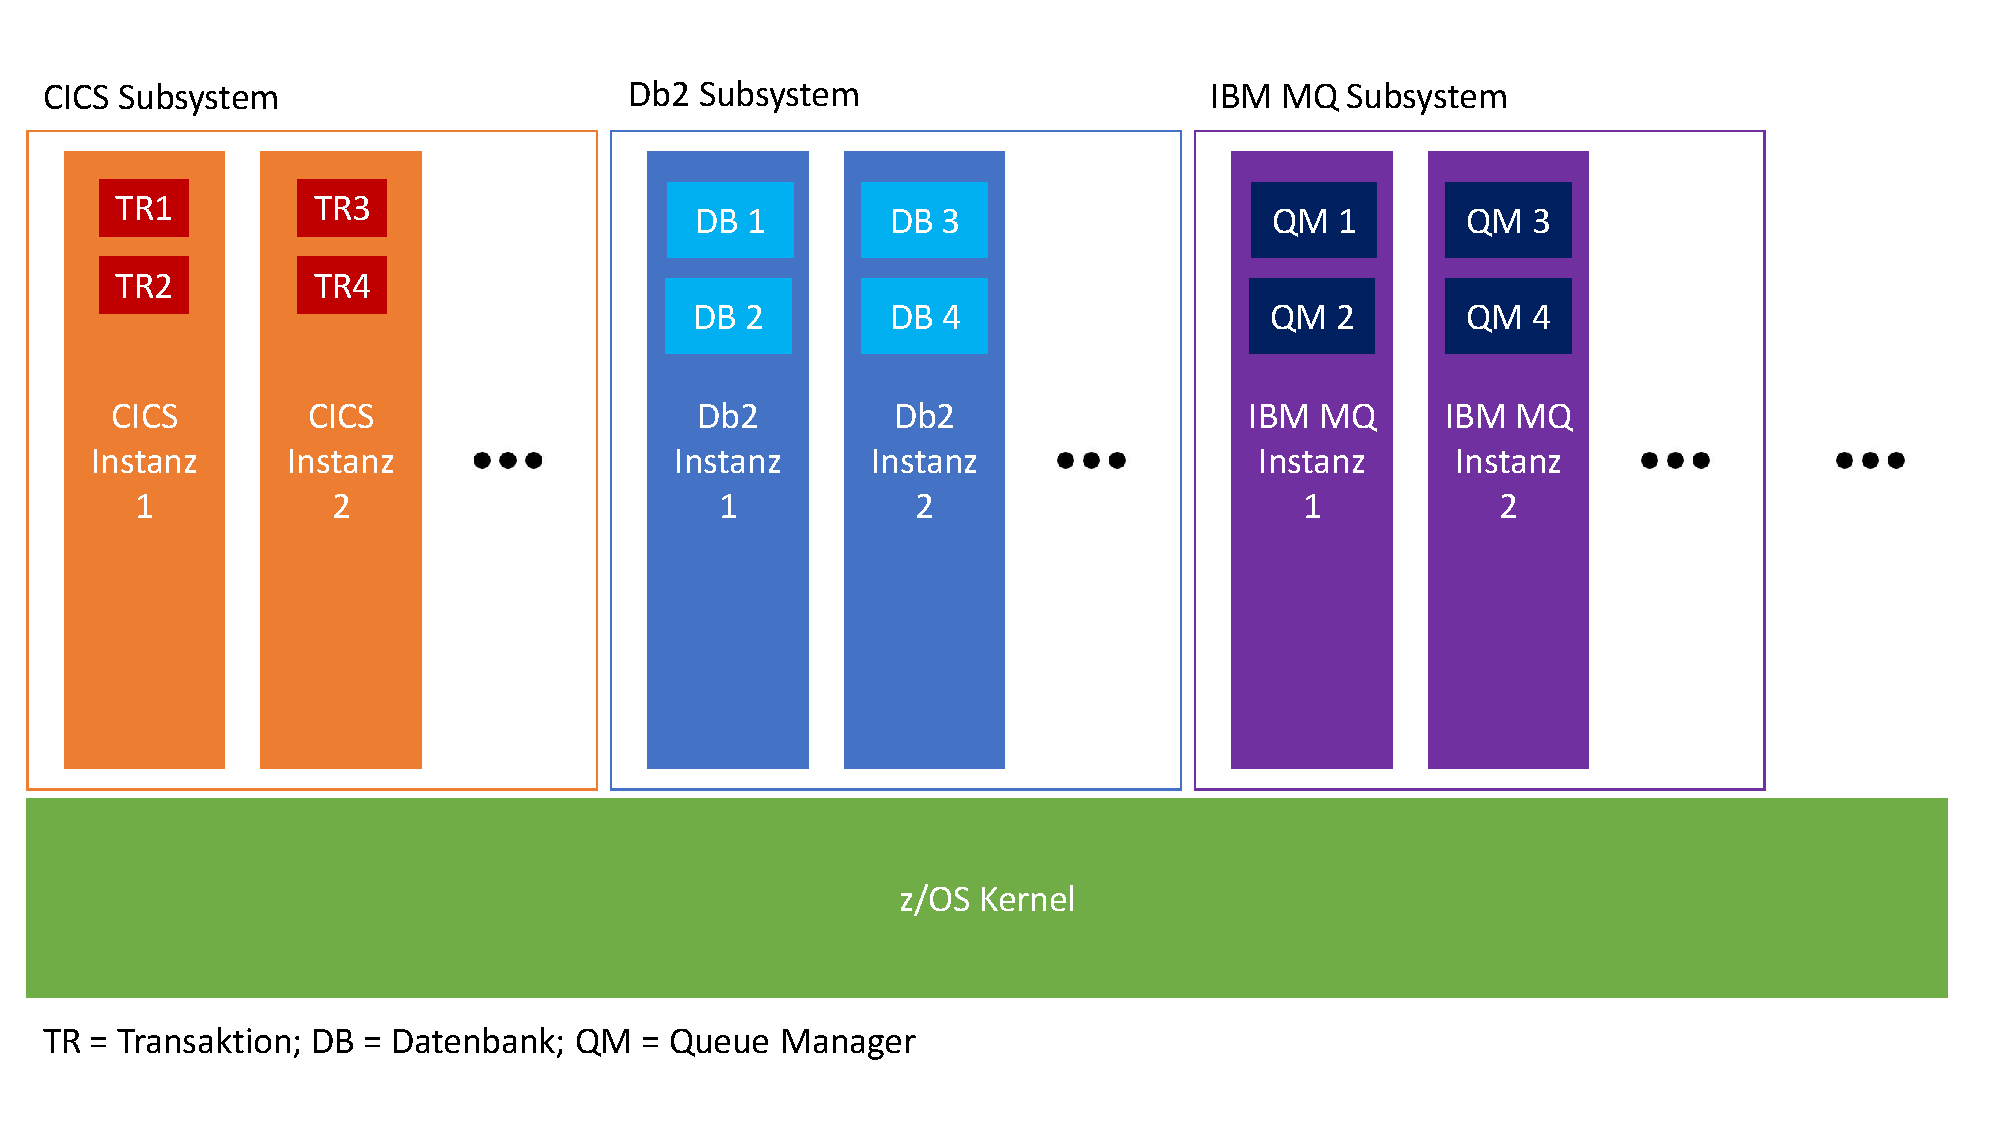
\includegraphics[width=\textwidth]{figures/architektur.pdf}
\caption{Architekturübersicht über die Subsysteme einer Stage bei DATEV eG}
\label{fig:archüber}
\end{figure}

\subsection{Customer Information Control System}\label{cics}
Das Customer Information Control System, kurz CICS, ist ein Applikationsserver für einen IBM-Großrechner mit Betriebssystem z/OS und damit eine IBM Middleware.
Ein Applikationsserver stellt eine Umgebung zur Verfügung, in der Anwendungen gehostet werden können.
Dabei kümmert sich dieser unter anderem um Transaktionalität, Webkommunikation und Sicherheit.
Hierfür stellen Applikationsserver eine API zur Verfügung.
CICS hat  gegenüber anderen Anwendungsservern (Kommentar: Beispiel? Websphere? Tomcat?)  den Vorteil, dass es verschiedene Programmiersprachen unterstützt.
Damit ist CICS ein Multi-Language Application Server und kann z.B. von COBOL, Assembler, Java und PLI Programmen genutzt werden.
So können Programme innerhalb einer Anwendung in der für ihren Use-Case am besten geeigneten Sprache implementiert werden, für die Kommunikation zwischen den verschiedenen Sprachen stellt  CICS mit seinem erwähnten API die Funktionalität zur Verfügung.
\cite{Rayns.2011}

Das CICS Subsystem einer Stage umfasst mehrere CICS Instanzen.

\subsubsection{CICS Instanz} 
Unter einer CICS Instanz ist ein einzelner Bereich, der auf dem z/OS Kernel aufsetzt, zu verstehen.
Dieser Bereich ist mittels einer eindeutigen CICS ApplicationID gekennzeichnet und kann darüber explizit verwaltet (Kommentar: ist das richtig?) werden.
Eine CICS Instanz verwaltet mehrere CICS Transaktionen.

Wenn in dieser Arbeit von dem CICS gesprochen wird, ist damit die CICS-Instanz  gemeint.

\subsubsection{CICS Transaktion}\label{subsec:trans}
Ein Businessablauf wird im CICS in einer Transaktion gekapselt.
Eine Transaktion kann mehrere Programme unterschiedlicher Programmiersprachen umfassen und wird über eine eindeutige \glqq TransaktionsID\grqq{} identifiziert..

Über die TransaktionsID wird der Ablauf gestartet.
Dies kann sowohl per Webanfrage oder per Messaging Queue als auch aus einem anderen Programm heraus oder manuell geschehen.
In der Transaktion werden alle Änderungen, die Programme an Ressourcen, wie zum Beispiel einer Datenbank oder Dateien tätigen, protokolliert.
So wird im Falle eines Fehlers die Möglichkeit eines Rollbacks (z.B. auf die in der Transaktion genutzte Datenbank) sichergestellt.
 \cite{Rayns.2011}

\subsection{Db2}\label{sssec:db2}
Db2 ist ein relationales Datenbanksystem, welches unter anderem als Subsystem eines z/OS Betriebssystems läuft.
Einer Stage können mehrere Datenbanksysteme, auch Instanzen genannt, zugeordnet werden.
In einer Instanz befinden sich die Datenbanken und Tabellen. (Kommentar: wie viele INstanzen haben wir in der Entwicklung?)

\subsection{IBM MQ}\label{sec:mq}
IBM MQ ist eine Messaging-Lösung der IBM.
Diese ermöglicht den asynchronen Datenaustausch zwischen Anwendungen mittels sogenannter Queues.
Alle IBM MQ Begrifflichkeiten, die in dieser Arbeit verwendet werden, werden im Folgenden erläutert.
\cite{Aranha.2013}

Das IBM MQ Subsystem einer Stage setzt sich aus einem oder mehreren Queue Managern zusammen.
Ein Queue Manager kann daher als IBM MQ Instanz gesehen werden.

\subsubsection{Queue Manager}
Bei einem Queue Manager handelt es sich um die zentrale Ressource eines IBM MQ Systems.
Er verwaltet  alle anderen IBM MQ Ressourcen.
Dazu gehören unter anderem die Speichersteuerung der Daten und die Wiederherstellung dieser im Falle eines Fehlers.
Desweiteren koordiniert er den Zugriff aller Anwendungen auf die Nachrichten in den von ihm verwalteten Queues.
Um hierbei die Konsistenz sicherzustellen, sorgt er für Locking und die notwendige Isolation der Queues.
\cite{Aranha.2013}

\subsubsection{Queues}
In Queues werden die Nachrichten, die von Programmen gesendet und gelesen werden gespeichert.
Es gibt verschiedene Arten von Queues, die im Kontext dieser Arbeit relevanten Queues sind folgende:

\paragraph{Die Local Queue.}~\\
Dabei handelt es sich um die einzige Queue Art, bei der die Nachrichten physikalisch gespeichert werden.
Die anderen Queue Arten nutzen als Basis immer eine Local Queue.

\paragraph{Initiation Queue}~\\
Die sogenannte \glqq Initiation Queue\grqq{} ist eine spezielle Art der Local Queue.
Diese dient dem Queue Manager dazu, unter bestimmten Bedingungen eine Trigger-Nachricht darauf zu schreiben.
Eine ander Local Queue kann so definiert sein, dass sobald eine Nachricht auf sie geschrieben wird, eine solche Trigger-Nachricht erzeugt wird.
Dies ermöglicht beispielsweise den use-case, dass Anwendungen nur starten, wenn wirklich Daten zum Verarbeiten vorhanden sind.
\cite{Aranha.2013}

\subsubsection{Process}
Für das Auslösen von Anwendungen wird nicht nur die Initiation Queue benötigt, sondern auch sogenannte \glqq Processes\grqq.
So muss der Local Queue, die den Start einer Anwendung auslösen soll, bei der Definition nicht nur die Initiation Queue bekannt gemacht werden, sondern auch ein Process.
Ein Process legt den \glqq Type\grqq{} und den Namen der zu startenden Anwendung fest.
Als \glqq Type\grqq{} können beispielhaft CICS oder auch WINDOWSNT für Windows unterstütze Plattformen genannt werden.
Ist der \glqq Type\grqq{} CICS,  muss der Name der Transaktion angegeben werden, für Windows Plattformen der Dateipfad der auszuführenden exe.
\cite{Aranha.2013}

\section{\glqq IBM Cloud Provisioning and Management for z/OS\grqq}\label{sec:tool}
Die Verwaltung von Subsystemen von z/OS ist eine hochspezialisierte, teilweise manuelle Tätigkeit.\footnote{Analyse des aktuellen Bereitstellungsprozesses, siehe in Absatz \ref{sec:aktbereit}}
Betreut werden die einzelnen Subsysteme über alle Stages hinweg von eigens dafür zuständigen Administratorenteams.
Die \glqq CICS Administration\grqq{} kümmert sich um alles rund um das CICS Subsystem.
Die \glqq Db2 Administration\grqq{} stellt Datenbanken und Tabellen auf Anfrage der Entwickler bereit.
Die \glqq IBM MQ Administration\grqq{} verwaltet die IBM MQ Ressourcen.
Um diese Aufgaben zu bewältigen, sind aktuell in erster Linie proprietäre Tools im Einsatz, die nicht der Erwartungshaltung an moderne Administrationstools entsprechen. (Kommentar: hier würde ich ein Bild einer "alten" Admin-Oberfläche als Beispiel zeigen, irgendeinen CICS-Dialog von den Admins, möglichst ISPF oder BMS )

Für die Automation dieser Prozesse bietet die IBM das \glqq IBM Cloud Provisioning and Management for z/OS\grqq{} an.
Dabei handelt es ich um ein bei der Installation von \glqq z/OS Management Facility\grqq{}\footnote{Siehe Absatz \ref{sssec:zosmf}}, kurz z/OSMF, mitgeliefertes Tool.
z/OSMF ist wiederum Teil der Standardauslieferung des Betriebssystems z/OS. 
Es soll z/OS-Administration über moderne Oberfläschen und APIs  ermöglichen.
(Kommentar: ich überlege gerade, ob der nächste Absatz nicht besser irgendwo anders aufgehängt werden sollte. Hier geht es um die Grundlagen des Tools, das was hier kommt ist quasi eine Bestätigung für die Relevanz der Forschungsfrage. Deshalb könnte man das so wie es ist vlt. noch umhängen - Zeilen 228 - 236)
z/OSMF (und damit auch \glqq IBM Cloud Provisioning and Management for z/OS\grqq) ist bei DATEV verfügbar, wird aber noch nicht flächendeckend eingesetzt. Die Administratoren kennen und vertrauen auf ihre herkömmlichen Tools, und sehen in der Umstellung immer auch Lernaufwand und Risiko.
\glqq IBM Cloud Provisioning and Management for z/OS\grqq{} ist auch außerhalb der DATEV e.G. kaum verbreitet. 
Deshalb besteht auch aus Sicht der IBM  Interesse an Erfahrungsberichten zur Nutzung von \glqq IBM Cloud Provisioning and Management for z/OS\grqq.
So wurde im Rahmen der neunzehnten \glqq AMC\grqq{}\footnote{Academic Mainframe Consortium e.V.} Tagung im IBM Client Center Böblingen am 16.01.2020 um ca. 14:30  (Kommentar: Uhrzeit??)  bei einem ca. 30 minütigen Vortrag ein Arbeitsstand dieser Arbeit vorgestellt.
Die Agenda der Veranstaltung ist im Anhang \ref{app:AMC} zu finden.
Der AMC e.V. ist ein Förderverein für die akademische Ausbildung auf dem Mainframe.\footnote{\cite{.23.2.2020}}
Neben Vertretern der IBM nahmen an der Tagung Vertreter von Hochschulen und verschiedenen Unternehmen teil.
Der Vortrag \glqq kam ja sehr gut an und hat auch später noch zu Gesprächen geführt\grqq\footnote{AMC Vorstand Ernst Lugert, 20.1.2020}. 
In den anschließenden Gesprächen wurde deutlich, dass sich neben der DATEV e.G. und der IBM auch andere Kundenfirmen für die automatisierte Provisionierung von z/OS Middleware mit \glqq IBM Cloud Provisioning and Management for z/OS\grqq{} interessieren, aber noch kaum Erfahrung in dem Umfeld besteht.

Bei \glqq IBM Cloud Provisioning and Management for z/OS\grqq{} stehen die sogenannten \glqq Templates\grqq{} im Mittelpunkt.
Mit Hilfe eines Templates können Instanzen erzeugt werden.
Diese Instanz kann eine oder mehrere verschiedene Subsystem-Instanzen enthalten.
Dabei steht sowohl eine schnelle Provisionierung, als auch Deprovisionierung von Instanzen durch den Entwickler im Vordergrund.
(Kommentar: auch die näcshten 2 Zeilen sind eine Annahme und können am ENde zur Bewertung herangezogen werden. d.h das könnte man auch in vlt. in die Analyse mit rein nehmen)
Mittels Templates läuft beides automatisiert, verlässlich, und ohne manuelle Abstimmungen ab.
Die Bereitstellung einer Instanz ist wiederholbar, so kann die Instanz z.B. im Fehlerfall sicher neugestartet werden und muss nicht langlebig gepflegt werden.
\\Das Template selbst ist eine Art "Verwaltungseinheit" und besteht aus drei Dateien:

\paragraph{\glqq Manifest-File\grqq} ~\\
Im  Manifest-File ist der Speicherpfad für das sogenannte \glqq Aktiondefinitionfile\grqq{} und das sogenannte \glqq Variableinputfile\grqq{} angegeben.
Erläuterungen zu diesen beiden Dateien folgen im Anschluss.
Da ein Template immer provisioniert werden kann, wird hier auch der Speicherpfad des Provisionierungsworkflows angegeben.
(Kommentar: ich finde die Formulierung schwierig, wäre es vlt. besser so: "für die Provisionierung des Templates ist auch die Angabe des Speicherpfads.... nötig)
\cite{.26.2.2020}

Ein Workflow ist über eine XML Datei, das sogenannte \glqq Workflowdefinitionfile\grqq, definiert.
Diese lässt sich grob in zwei Teile untergliedern:
\begin{itemize}
\item Variablendefinition
\item Steps
\end{itemize}
In der Variablendefinition werden, wie der Name schon sagt, alle Variablen, die für diesen Workflow notwendig sind definiert.

Ein Step beschreibt einen Teilablauf eines Workflows.
Ein Workflow kann aus mehreren Steps bestehen.
Die Steps werden in Definitionsreihenfolge ausgeführt.
Allerdings können Bedingungen für die Durchführung eines Steps definiert werden.
So ist es beispielsweise möglich, einen Step nur durchzuführen, wenn eine bestimmte Variable einen bestimmten Wert besitzt.
Innerhalb eines Steps können sowohl interne und externe Scripte als auch JCLs und somit z/OS Programme ausgeführt werden.
Darüber hinaus besteht die Möglichkeit REST-Calls auszuführen.
Durch ein XML Schema wird sichergestellt, dass das Workflowdefinitionfile keine syntaktischen Fehler beinhaltet.
Sowohl die Variablendefinition als auch die Steps können in externe XML Dateien ausgelagert werden.
Dadurch können Variablen an einer Stelle im Template definiert und in alle Workflowdefinitionfiles aufgenommen werden.
\cite{Rotthove.2018}

Zusätzlich kann in dem Manifest-File eine Beschreibung des Templates hinzugefügt werden.
\cite{.26.2.2020}
\paragraph{\glqq Aktiondefinitionfile\grqq} ~\\
Weitere optionale Aktionen, die ein Anwender mit einer Instanz eines Templates durchführen kann, werden in dem Aktiondefinitionfile festgelegt.
Standardmäßig handelt es sich dabei um folgende Aktionen.
Die Begriffe werden am Beispiel einer Template-Instanz, die eine Datenbank provisioniert, erläutert.
\begin{itemize}
\item check\_status\\
Prüft den Status der Template-Instanz, beispielsweise ob die Datenbank erreichbar ist.
\item start\\
Welche Schritte sollen beim Starten der Template-Instanz durchgeführt werden.
Beispielsweise die Erzeugung von Tabellen.
\item stop\\
Welche Schritte sollen beim Stoppen der Template-Instanz durchgeführt werden.
Beispielsweise das Löschen von Tabellen.
\item deprovisioning\\
Welche Schritte sollen beim Entfernen der Template-Instanz durchgeführt werden.
Üblicherweise wird die Template-Instanz zunächst gestoppt, am Beispiel der Datenbank ist dies nicht notwendig, da beim Löschen der Datenbank automatisch die Tabellen auch gelöscht werden.
\end{itemize}

Neben den Workflowdefinitionfiles muss in einer Aktion auch der Pfad für das sogenannte \glqq Variableinputfile\grqq{} angegeben sein.
\cite{.26.2.2020}

\paragraph{\glqq Variableinputfile\grqq}\label{par:variable} ~\\
In dieser Datei werden den in der Workflowdefinitionfile definierten Variablen Werte zugewiesen.
Somit kann das Template für spezifische Anforderungen, z.B. einer speziellen Anwendung,  konfiguriert werden.

Für die Provisionierung eines Templates müssen diesem eine sogenannte \glqq Domain\grqq{} und ein \glqq Tenant\grqq{} zugewiesen werden.
Unter einer \glqq Domain\grqq{} ist ein System zu verstehen, das Systemressourcen in Ressourcenpools gliedert.
\glqq Tenants\grqq{} sind die dazugehörigen Rechtegruppen, die dem Anwender den Zugriff auf und die Nutzung von zugeordneten Templates ermöglicht.
\cite{Rotthove.2018}

\glqq IBM Cloud Provisioning and Management for z/OS\grqq{} umfasst zwei Lösungen, \glqq z/OS Management Facility\grqq\footnote{siehe Absatz \ref{sssec:zosmf}} und \glqq z/OS Provisioning Toolkit\grqq\footnote{siehe Absatz \ref{sssec:zospt}}.

\subsection{z/OS Management Facility}\label{sssec:zosmf}
Der Funktionsumfang von z/OS Management Facility, kurz z/OSMF, umfasst Systemmanagementfunktionen
in einer browserbasierenden Benutzeroberfläche, dargestellt in Abbildung \ref{fig:zosmf_welcome}.
Zu diesen Funktionen zählt auch die Verwaltung von Workflows und Templates.

\begin{figure}[h]
\centering
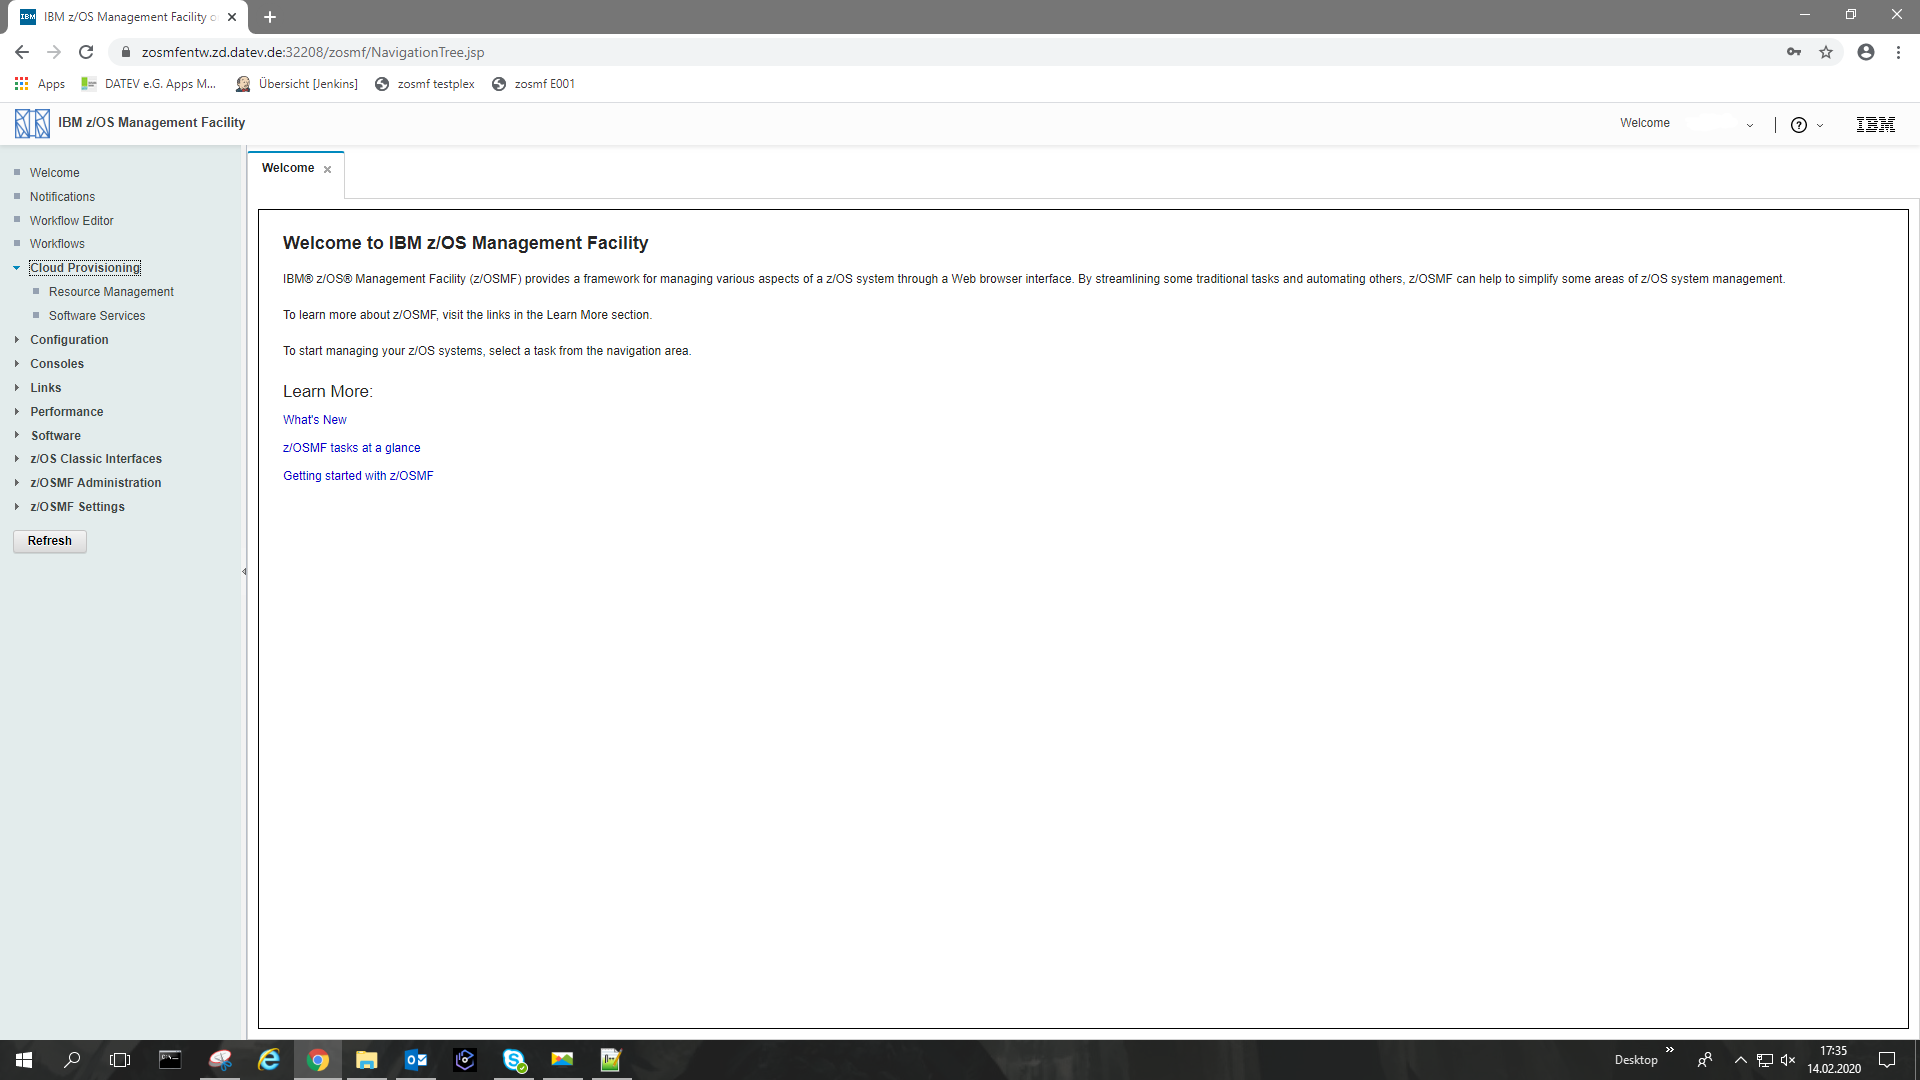
\includegraphics[width=\textwidth]{figures/zosmf.png}
\caption{z/OSMF Willkomens Ansicht}
\label{fig:zosmf_welcome}
\end{figure}

Die linke Seite der Abbildung \ref{fig:zosmf_welcome} zeigt den Umfang der z/OSMF  Funktionen.
Für diese Arbeit besitzt nur der Menüpunkt \glqq Cloud Provisioning\grqq{} Relevanz .
Unter diesem Punkt sind die Funktionalitäten von \glqq IBM Cloud Provisioning and Management for z/OS\grqq{} zu finden, und der Begriff  \glqq z/OSMF\grqq{} wird im folgenden synonym für diese Lösung verwendet
\cite{Rotthove.2018}

Unter dem Punkt \glqq Resource Management\grqq{} werden die \glqq Domains\grqq{} und \glqq Tenants\grqq{} verwaltet.
Zur Verwaltung der Templates und Template-Instanzen kommen die \glqq Software Services\grqq{} zum Einsatz.
Dort können neue Templates über die Manifest-Files hinzugefügt werden.
Es folgt, wie oben beschrieben, die Zuweisung einer \glqq Domain\grqq{} und eines \glqq Tenants\grqq{}.
Anschließend kann das Template, falls es keine Fehler beinhaltet, veröffentlicht werden.
Es ist zu empfehlen vorher einen \glqq Test Run\grqq{} durchzuführen.
Dabei wird eine Instanz testweise provisioniert.
Diese Test-Template-Instanz verhält sich genauso wie eine Instanz, die aus einem veröffentlichten Template erzeugt wurde. 
Somit können das Template und die in der Aktiondefintionfile definierten Aktionen vor der Veröffentlichung getestet werden.
\cite{Rotthove.2018}


\subsection{z/OS Provisioning Toolkit}\label{sssec:zospt}
Das z/OS Provisioning Toolkit, kurz z/OSPT bietet für das Provisionieren von Laufzeitumgebungen ein Kommandozeileninterface für die Bereitstellung und das Verwalten von Templates bzw. \glqq Images\grqq{} sowie das Starten von Instanzen an. 
z/OSPT orientiert sich an der Docker Commandline und spricht von Containern (auch wenn es in z/OS diese nicht gibt) und Images.
Zur Erläuterung werden die Begriffe hier  gegenüber gestellt.

\paragraph{\glqq Docker-Images\grqq}~\\

Ein Docker-Image beschreibt die Vorlage für einen Docker-Container und beinhaltet alle Elemente, die für die Ausführung einer Anwendung als Container benötigt werden, so wie den Code, Konfigurationsdateien, Umgebungsvariablen, Bibliotheken und die Laufzeitumgebung.

\paragraph{\glqq Docker-Container\grqq}~\\
Mit dem Kommandozeilenbefehl \glqq docker run\grqq{} wird aus einem Docker-Image ein Docker-Container erzeugt.
Ein Docker-Container beschreibt somit eine lauffähige Instanz eines Docker-Images.
\cite{Vohra.2016}

Im Vergleich dazu sind die Definitionen in z/OSPT folgende:
\paragraph{\glqq z/OSPT-Images\grqq}~\\
Grundsätzlich ist ein z/OSPT-Image einem Docker-Image nicht unähnlich.
Auch ein z/OSPT Image ist für die Erzeugung eines z/OSPT Containers zuständig und beinhaltet alle ELemente, die die ANwendung zur Laufzeit benötigt
Es verknüpft ein Template mit den enthaltenen Dateien (Actiondefinitionfile, Variableinputfile und die Manifest-File) mit einer weiteren nicht im Template enthaltenen Konfigurationsdatei, der sogenannten \glqq zosptfile\grqq.
In dieser muss der Name des zugrundeliegenden Templates angegeben werden.
Danach ist es möglich, die Werte aus der Variableinputfile zu überschreiben und so das Verhalten der Template-Instanz zu verändern.
Dadurch kann ein Template mit spezifischen Änderungen provisioniert werden, ohne dass ein neues Template erzeugt werden muss.

\paragraph{\glqq z/OSPT-Container\grqq}~\\
Die Beziehung zwischen einem z/OSPT-Container und einem z/OSPT-Image ist die gleiche wie zwischen einem Docker-Container und einem Docker-Image.
Ein z/OSPT-Container entspricht einer Template-Instanz, die mit Hilfe eines z/OSPT-Images gestartet wurde.

Um nun einen z/OSPT-Container bereitzustellen, muss ein Template zur Verfügung stehen.
Es ist von Vorteil, wenn diesem über die z/OSMF Oberfläche bereits eine Domain und ein Tenant zugewiesen worden sind, dies ist ohne die z/OSMF Oberfläche nicht ohne weiteres möglich. (Kommentar: das ist doch eine Erkenntnis aus der Analyse oder Realisierung. Das gehört hier eigentlcih noch nicht hin, oder? kannst du darauf nicht verweisen?)
Anschließend kann mittels des Konsolenbefehls \glqq zospt build\grqq{} und der Angabe des Pfades der zosptfile ein Image erzeugt werden.
Wird nun der \glqq zospt run\grqq-Befehl ausgeführt, wird ein z/OSPT-Container erzeugt (entspricht dem Provisionieren einer Template-Instanz) und gestartet (nur wenn die start-Aktion in der Actiondefinitionfile definiert wurde).
Der Status von vorhanden Instanzen und Container kann ebenfalls mittels Kommandozeilenbefehlen abgefragt werden.
\cite{IBM.2019b}
In Abbildung \ref{fig:zospt_help} werden die möglichen Kommandozeilenbefehle mittels des Befehls \glqq zospt -h\grqq{} in einem Kommandofenster angezeigt. 
\begin{figure}[h]
	\centering
	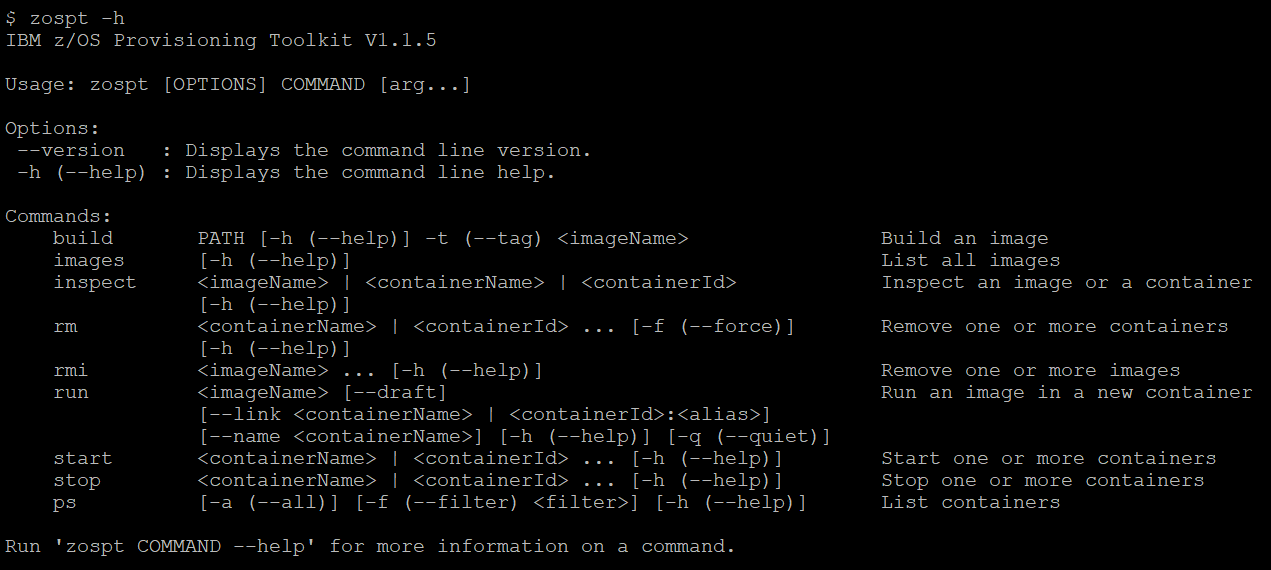
\includegraphics[width=\textwidth]{figures/zospt_help_putty.png}
	\caption{z/OSPT mögliche Kommandozeilenbefehle}
	\label{fig:zospt_help}
\end{figure}
